    \documentclass[11pt]{article}
    %	options include 12pt or 11pt or 10pt
    %	classes include article, report, book, letter, thesis
    
    \title{HW4}
    \author{Shane Drafahl}
    \date{16 October ,2017}
    \usepackage{graphicx}
    \usepackage{epstopdf}
    \usepackage{graphics}

    \begin{document}
    \maketitle

     1. For union This means that the language accepted by the turring machine 
     is just a subset of a language that is already accepted. To biuld a turring machine
     I would just use double sided tape and would take a string from both languages that
     are unioned and put one on each side of the tape. I would then takes turns with 
     the algorithm on each perspective language on both sides of the tape. If both sides of the tape
     are accepted then the language is valid.

     $ \newline $
        Here is a small example of what the tape could look like. Where $ a_{n} $ is from one language
        and $ b_{n} $ is from another.
     $ \newline $

    \begin{figure}[!htb]
        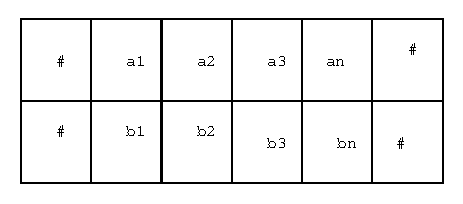
\includegraphics[scale=.7]{./turring.eps}
    \end{figure}

    $ \newline $

    For intersection I will still be using two sides of the tape but in this case if either side
    is accepted then the whole thing is accepted.

    $ \newline $

    \begin{figure}[!htb]
        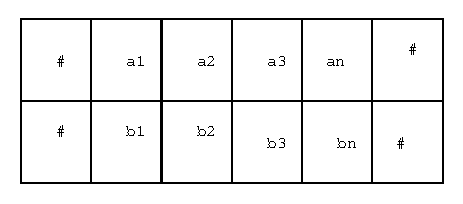
\includegraphics[scale=.7]{./turring.eps}
    \end{figure}

    $ \newline $

    For reversal I would simply copy the input from one side of the tape to the other in reverse
    order. I would then have the original accepts either side of the tape we know it is accepting.

    $ \newline $

    2. Turing-acceptable languages are closed under concatentation. Assuming we have two turring
    machines that are acceptable we can put a deliminator between two strings from the 
    two langauges on either side of the deliminator. On the left side of the deliminator
    we will use one turring machine and after the deliminator we will use the other one.
    If the left side or the right side is not acceptable the whole thing will not be acceptable.

    $ \newline $

    3. a 

    $ \newline $

    For this turring machine $ \Delta (a_{n}, b_{n}) $ = $ (a_{n + 1}, R) $ (GO RIGHT)
    $ \newline $
    $ \Delta (a_{n}, b_{n}) $ = $ (a_{n + 1}, L) $ (GO LEFT)
    $ \newline $
    b. 
    $ \newline $
    
    This machine M1 accepts pushdown automata's. We can prove this by showing that 
    $ M(L) \subset M1(L) $ where the pushdown automata is the subset of the given subset.
    This is true because if we give all languages that are accepted by M to M1 they would be
    accepted. We know this because the only difference is that M1 has an extra stack. 
    This argument is symetric of why a DFA is a subset of FA. For turring machines
    we can show it is equivelant. We can simulate the TM if we put all the contents left of the 
    head in the first stack and to the right we put all the elements in the right stack. To 
    go left we pop from the left stack and vice versa with the right stack. Up and down
    is simulated because we can put multiple dimensions of tape onto the same side of tape
    by putting in a pattern. For example every odd element could be for the back side of the
    tape and every even is on the front. In the other direction a turring machine can simply use 
    two dimensions or two peices of tape to represent each of the stacks and a third tape for
    the K finite states.
    



    \end{document}